
\documentclass[12pt]{report}
\usepackage[a4paper]{geometry}
\usepackage[myheadings]{fullpage}
\usepackage{fancyhdr}
\usepackage{lastpage}
\usepackage{graphicx, wrapfig, subcaption, setspace, booktabs}
\usepackage[T1]{fontenc}
\usepackage[font=small, labelfont=bf]{caption}
\usepackage{fourier}
\usepackage[protrusion=true, expansion=true]{microtype}
\usepackage[english]{babel}
\usepackage{sectsty}
\usepackage{url, lipsum}
\usepackage{color}
\usepackage{hyperref}
\usepackage{array}
\usepackage{supertabular}
\usepackage{hhline}
\usepackage{enumitem}
\usepackage[T1]{fontenc}
\usepackage[utf8x]{inputenc}
\usepackage{graphicx}
\newcommand{\HRule}[1]{\rule{\linewidth}{#1}}
\renewcommand{\theenumii}{\arabic{enumii}.}
\addto\captionsenglish{
  \renewcommand{\contentsname}
    {Innhold}
}
\onehalfspacing
\setcounter{tocdepth}{5}
\setcounter{secnumdepth}{5}
%-------------------------------------------------------------------------------
% HEADER & FOOTER
%-------------------------------------------------------------------------------
\pagestyle{fancy}
\fancyhf{}
\setlength\headheight{15pt}
\fancyhead[L]{Team D} 
\fancyhead[R]{Universitetet i Bergen}
\fancyfoot[R]{Page \thepage\ of \pageref{LastPage}}
%-------------------------------------------------------------------------------
% TITLE PAGE
%-------------------------------------------------------------------------------
\begin{document}
\title{ \normalsize \textsc{}
		\\ [2.0cm]
		\HRule{0.5pt} \\
		\LARGE \textbf{\uppercase{Bilspill}}
		\HRule{2pt} \\ [0.5cm]
		\normalsize \today \vspace*{5\baselineskip}}
\date{}
\author{
		Team D  \\ 
		Universitetet i Bergen \\
		Informatikk }
\maketitle
\tableofcontents
\newpage
%-------------------------------------------------------------------------------
% Section title formatting
\sectionfont{\scshape}
%-------------------------------------------------------------------------------
%-------------------------------------------------------------------------------
% BODY
%-------------------------------------------------------------------------------
\section*{Bruksmønstertekst:}
\addcontentsline{toc}{section}{Bruksm{\o}nstertekst:}
\textbf{Tittel}: Få høyest mulig score
\bigskip \\
\textbf{Akt{\o}rer}: Spiller, System
\bigskip \\
\textbf{Prim{\ae}rakt{\o}r}: Spiller
\bigskip \\
\textbf{Tid}: Varierende, avhengig av spillers prestasjon
\bigskip \\
\textbf{M{\aa}l}: Få høyest mulig highscore før man går tom for bensin
\bigskip \\
\textbf{Pre-conditions:} Spillet er startet på en datamaskin
\subsubsection*{Hovedflyt:}
\begin{enumerate}
\item Systemet viser startmeny
\item Spiller velger å starte spillet
\item Systemet startet spillet
\item Spiller styrer bil med venstre/høyre piltast
\item Systemet flytter bilen i takt med tastetrykk
\item Spiller unngår hindre
\item Spiller kjører på folk
\item Systemet legger til én mynt i spillerens inventar for hver person som blir påkjørt
\item Spiller kjører over en bensintank
\item Systemet legger til bensinen i en "counter", som gjør at spilleren kan kjøre lengre
\item Spiller går tom for bensin
\item Systemet stopper spillet
\item Systemet lagrer spillers score
\item Systemet viser spillers score og highscore
\item Systemet viser startmeny
\end{enumerate}
\pagebreak
\subsubsection*{Alternative handlinger:}
\begin{enumerate}[label=\Alph*]
\item 
\bigskip
\begin{enumerate}
\item @1 Spiller klikker på oppgradering
\item Systemet viser spiller mulige oppgraderinger 
\item Spiller kjøper oppgradering
\item Systemet oppgraderer bilen
\item Spiller klikker seg tilbake til startmenyen
\item Gjenoppta @1
\end{enumerate}
\item 
\bigskip
\begin{enumerate}
\item @1 Spiller trykker på innstillingsknapp
\item Systemet viser spiller mulige innstillinger for spillet
\item Spiller endrer innstillinger
\item Systemet lagrer instillingene
\item Gjenoppta @1
\end{enumerate}
\item
\bigskip
\begin{enumerate}
\item @3, 4, 5 Spiller pauser spiller
\item Systemet viser en pauseskjerm
\item Spiller velger å avslutte spillet
\item Gjenoppta @13
\end{enumerate}
\item
\bigskip
\begin{enumerate}
\item @3, 4, 5 Spiller pauser spiller
\item Systemet viser en pauseskjerm
\item Spiller velger å gjenoppta spillet
\item Gjennoppta @3
\end{enumerate}
\end{enumerate}
\pagebreak
\section*{Bruksmønsterdiagram:}
\addcontentsline{toc}{section}{Bruksm{\o}nsterdiagram:}
\vspace{4cm}
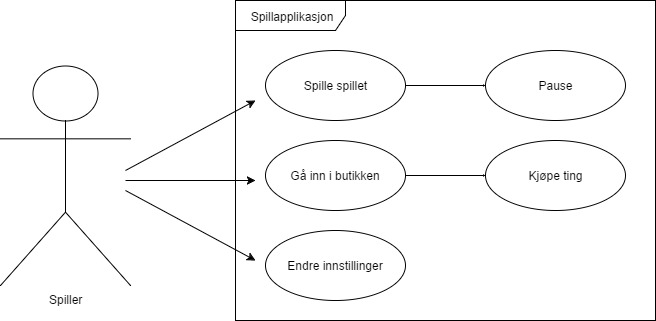
\includegraphics[width=0.8\textwidth,natwidth=500,natheight=642]{use_case_diagram_b.jpg}
\end{document}